% IEEE conference paper (IEEEtran). Edit this file directly.
% Overleaf: New Project > Upload Project, then Menu > Compiler: XeLaTeX
% (XeLaTeX is needed for the Devanagari examples; IEEEtran.cls ships with TeX Live).
\documentclass[conference]{IEEEtran}
\usepackage{fontspec}
\setmainfont{TeX Gyre Termes}
\newfontfamily\dev[Script=Devanagari]{Noto Serif Devanagari}
\usepackage{amsmath}
\usepackage{booktabs}
\usepackage{tabularx}
\usepackage{xcolor}
\usepackage{tikz}
\usetikzlibrary{arrows.meta}
\usepackage{pgfplots}
\pgfplotsset{compat=1.17}
\usepackage[hidelinks]{hyperref}
\definecolor{navy}{HTML}{12304A}
\definecolor{teal}{HTML}{1CA69A}
\definecolor{c1CA69A}{HTML}{1CA69A}
\definecolor{c9AA5B1}{HTML}{9AA5B1}
\definecolor{c12304A}{HTML}{12304A}
\begin{document}

\title{Evidence-Linked Screening Forms from Hindi Clinical Consultations with Cross-Lingual Entity Projection}

\author{\IEEEauthorblockN{Soumya Ranjan Behera}
\IEEEauthorblockA{Enrollment ID: 230102\\\textit{Natural Language Processing Final Project (Industry Track)}}
\and
\IEEEauthorblockN{Sourabh Sarkar}
\IEEEauthorblockA{Enrollment ID: 230081\\\textit{Natural Language Processing Final Project (Industry Track)}}
\and
\IEEEauthorblockN{Manish Kumar}
\IEEEauthorblockA{Enrollment ID: 230152\\\textit{Natural Language Processing Final Project (Industry Track)}}
\and
\IEEEauthorblockN{Prashant Kumar}
\IEEEauthorblockA{Enrollment ID: 230101\\\textit{Natural Language Processing Final Project (Industry Track)}}
\and
\IEEEauthorblockN{Monu Kumar}
\IEEEauthorblockA{Enrollment ID: 230113\\\textit{Natural Language Processing Final Project (Industry Track)}}}

\maketitle

\begin{abstract}
Oncology screening consultations in India are often conducted in Hindi or Hindi–English code-mixed speech, while the screening record is a structured English form. We present an academic prototype that converts consultation audio into an evidence-linked screening form. Whisper produces a Hindi transcript and an English translation; a rule- and lexicon-based layer segments question–answer turns, recognises 22 clinical entity types, assigns a four-state assertion (PRESENT, ABSENT, POSSIBLE, UNKNOWN) and maps concepts to SNOMED-CT and UMLS identifiers. Every English entity is then projected back to its Hindi source words using Whisper timestamps and a phonetic consonant-skeleton matcher that tolerates noisy ASR spellings. On four consultations with reference forms (56 assertion fields), the system answers 39.3\% of the fields and is correct on all 22 it answers. A trivial “always absent” baseline reaches 96.4\% exact agreement with zero recall of positive findings, which shows that accuracy alone is uninformative on this class-imbalanced data. Clause-level question detection removes all 16 clinician-question mentions that were previously labelled as patient findings, and phonetic matching raises word-level Hindi alignment from 14.8\% to 23.3\% of entities. An error-propagation analysis attributes 74\% of the 34 unanswered fields to speech recognition and translation rather than to the language-processing stages.
\end{abstract}

\begin{IEEEkeywords}
Clinical NLP, code-mixed speech, Hindi, Whisper, assertion detection, cross-lingual annotation projection, information extraction, oncology screening
\end{IEEEkeywords}

\section{Introduction}
Cancer screening camps in India record each patient on a structured paper form: demographics, risk factors such as tobacco use, family history, general warning signs and an oral examination. The interview itself is spoken, usually in Hindi or in Hindi–English code-mixed speech, and the clinician later transcribes the answers by hand. Turning such conversations directly into structured records is an instance of \emph{ambient clinical documentation}~\cite{aci}, here in a low-resource, code-mixed setting and with a form rather than a free-text note as the target.

Four properties make the task harder than transcription. First, conversational Hindi ASR is noisy, and Whisper is known to hallucinate fluent but unspoken text on long or quiet audio~\cite{careless}. Second, code-mixing produces inconsistent spellings of the same word: the English loan word \emph{cancer} appears in our transcripts as {\dev कैंसर, कानसर, खंसर} and {\dev खणसर}. Third, clinical meaning depends on context: a term can be negated, hedged, or uttered by the clinician inside a question rather than reported by the patient~\cite{negex,context}. Fourth, an unanswered question is not a denial; silently recording “no” for every unanswered field invents negative findings.

This paper describes the system our team built for the course project and makes four contributions:

\begin{enumerate}
\item An end-to-end pipeline from consultation audio to a screening form in which every populated field carries its source question and answer, and unanswered fields remain UNKNOWN rather than ABSENT.
\item A cross-lingual entity projection method that links each English entity to its Hindi source span using Whisper timestamps and a phonetic consonant skeleton, with detection of hallucinated Hindi segments.
\item An evaluation that reports coverage, selective accuracy and positive recall next to trivial baselines, together with an ablation study and a stage-wise error-propagation analysis.
\item A local review dashboard and an annotation tool with inter-annotator agreement measurement, so that named-entity gold data can be built independently of the system's predictions.
\end{enumerate}

\section{Related Work}
\subsection{Speech Recognition}
Whisper~\cite{whisper} is a multilingual encoder–decoder ASR model trained on 680k hours of weakly supervised audio; it can transcribe Hindi or translate it directly into English. Koenecke \emph{et al.}~\cite{careless} documented that Whisper inserts hallucinated content, often as repetition loops. We measure the same failure on our recordings and filter it before alignment.

\subsection{Clinical Information Extraction and Assertion}
MetaMap~\cite{metamap} and cTAKES~\cite{ctakes} map clinical text to UMLS~\cite{umls} concepts with dictionaries and rules. NegEx~\cite{negex} detects negated findings with trigger phrases and a fixed window; ConText~\cite{context} adds hypothetical and historical status and terminates a trigger's scope at clause boundaries. The 2010 i2b2/VA challenge~\cite{i2b2} standardised assertion classes such as present, absent and possible. Our assertion component is ConText-style and uses four states, where UNKNOWN marks a fact that the conversation did not establish.

\subsection{Cross-Lingual Entity Projection}
Annotation projection transfers labels from one language to another through word alignment~\cite{yarowsky}; translate-then-project approaches apply it to NER in low-resource languages~\cite{mayhew}, and embedding-based aligners such as SimAlign~\cite{simalign} remove the need for parallel training data. Our setting differs in that the two “parallel” texts are two ASR outputs of the same audio. Timestamps therefore provide the sentence alignment, and only the word alignment must be inferred.

\subsection{Neural NER and Indian Languages}
GLiNER~\cite{gliner} performs zero-shot NER from natural-language type descriptions and serves as our neural comparison point. MuRIL~\cite{muril} is a multilingual encoder for Indian languages, including transliterated text, and is the natural basis for future native-Hindi NER.

\section{Data}
The project data are five recorded screening consultations, referred to here as C1–C5, together with scanned paper forms transcribed into JSON. Case identifiers match for four consultations (C2–C5); C1 has audio but no reference form, and one reference form has no recording. Every form contributes 14 assertion fields (family history of cancer, past tobacco or alcohol use, current tobacco use, seven general warning signs and four oral-screening criteria) plus age and weight. Table~\ref{tab:data} summarises the material.

\begin{table}[!t]
\centering\footnotesize
\caption{Dataset and transcript statistics}\label{tab:data}
\begin{tabular}{llrrr}
\toprule
\textbf{Case} & \textbf{Ref. form} & \textbf{Hindi seg.} & \textbf{English seg.} & \textbf{Entities} \\
\midrule
C1 & no & 65 & 95 & 41 \\
C2 & yes & 56 & 74 & 30 \\
C3 & yes & 29 & 70 & 28 \\
C4 & yes & 80 & 70 & 43 \\
C5 & yes & 31 & 85 & 34 \\
\midrule
Total & 4 & 261 & 394 & 176 \\
\bottomrule
\end{tabular}
\end{table}

The reference labels are highly imbalanced: of the 56 scorable assertion fields, 54 are ABSENT and only 2 are PRESENT (both family history); there are no POSSIBLE labels, and all 11 symptom fields are ABSENT. This property dominates the interpretation of the results in Section VI.

\section{System}
Fig.~\ref{fig:arch} shows the pipeline. It is implemented in Python using only the standard library; the only external component is the Whisper command-line tool.

\begin{figure}[!t]
\centering
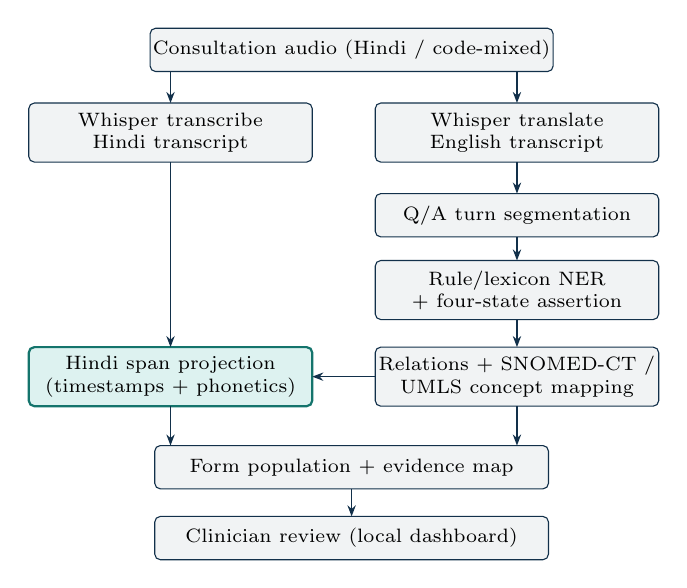
\begin{tikzpicture}[x=1cm,y=1cm,font=\scriptsize]
\node[fill=navy!6,draw=navy,rounded corners=2pt,minimum width=5.0cm,minimum height=0.55cm,align=center,inner sep=1pt] (audio) at (4.2,0.0) {Consultation audio (Hindi / code-mixed)};
\node[fill=navy!6,draw=navy,rounded corners=2pt,minimum width=3.6cm,minimum height=0.75cm,align=center,inner sep=1pt] (hi) at (1.9,-1.05) {Whisper transcribe\\Hindi transcript};
\node[fill=navy!6,draw=navy,rounded corners=2pt,minimum width=3.6cm,minimum height=0.75cm,align=center,inner sep=1pt] (en) at (6.3,-1.05) {Whisper translate\\English transcript};
\node[fill=navy!6,draw=navy,rounded corners=2pt,minimum width=3.6cm,minimum height=0.55cm,align=center,inner sep=1pt] (qa) at (6.3,-2.1) {Q/A turn segmentation};
\node[fill=navy!6,draw=navy,rounded corners=2pt,minimum width=3.6cm,minimum height=0.75cm,align=center,inner sep=1pt] (ner) at (6.3,-3.05) {Rule/lexicon NER\\+ four-state assertion};
\node[fill=navy!6,draw=navy,rounded corners=2pt,minimum width=3.6cm,minimum height=0.75cm,align=center,inner sep=1pt] (rel) at (6.3,-4.15) {Relations + SNOMED-CT /\\UMLS concept mapping};
\node[fill=teal!15,draw=teal!70!black,thick,rounded corners=2pt,minimum width=3.6cm,minimum height=0.75cm,align=center,inner sep=1pt] (proj) at (1.9,-4.15) {Hindi span projection\\(timestamps + phonetics)};
\node[fill=navy!6,draw=navy,rounded corners=2pt,minimum width=5.0cm,minimum height=0.55cm,align=center,inner sep=1pt] (form) at (4.2,-5.3) {Form population + evidence map};
\node[fill=navy!6,draw=navy,rounded corners=2pt,minimum width=5.0cm,minimum height=0.55cm,align=center,inner sep=1pt] (review) at (4.2,-6.2) {Clinician review (local dashboard)};
\draw[-{Stealth[length=4pt]},navy,semithick] (1.9,-0.275) -- (1.9,-0.675);
\draw[-{Stealth[length=4pt]},navy,semithick] (6.3,-0.275) -- (6.3,-0.675);
\draw[-{Stealth[length=4pt]},navy,semithick] (6.3,-1.425) -- (6.3,-1.825);
\draw[-{Stealth[length=4pt]},navy,semithick] (6.3,-2.375) -- (6.3,-2.675);
\draw[-{Stealth[length=4pt]},navy,semithick] (6.3,-3.425) -- (6.3,-3.775);
\draw[-{Stealth[length=4pt]},navy,semithick] (1.9,-1.425) -- (1.9,-3.775);
\draw[-{Stealth[length=4pt]},navy,semithick] (4.5,-4.15) -- (3.7,-4.15);
\draw[-{Stealth[length=4pt]},navy,semithick] (1.9,-4.525) -- (1.9,-5.025);
\draw[-{Stealth[length=4pt]},navy,semithick] (6.3,-4.525) -- (6.3,-5.025);
\draw[-{Stealth[length=4pt]},navy,semithick] (4.2,-5.575) -- (4.2,-5.925);
\end{tikzpicture}
\caption{System pipeline. NLP runs on the English translation; the highlighted stage projects each entity back to the Hindi transcript.}\label{fig:arch}
\end{figure}

\subsection{Speech Recognition}
\texttt{whisper-cli} with the multilingual \emph{small} GGML model runs twice per recording: once transcribing Hindi and once translating to English. Both passes keep segment-level start and end times in milliseconds, which later serve as the bridge between the two languages.

\subsection{Question–Answer Segmentation}
There is no speaker diarization, so the clinician's turns are inferred. A segment is a question when it ends in “?” or begins with an interrogative cue (\emph{what}, \emph{do you}, \emph{have you}, \emph{is there}, \emph{any}, \ldots{}), because ASR frequently drops question marks. Each question is grouped with the following non-question segments as its answer, and a segment containing both an inline question and its answer is split at the question mark.

\subsection{Entity Recognition and Concept Mapping}
Regular expressions and lexicons recognise 22 entity types, covering demographics (age, education, occupation, income), anthropometrics, symptoms, oral signs, cancer types, tobacco and alcohol risk factors, diet, physical activity, family members and durations. A local dictionary maps 39 clinical terms to SNOMED-CT codes and UMLS CUIs. The component is a transparent rule system, not a trained model; Section V-E describes how we evaluate it.

\subsection{Four-State Assertion}
Each clinical mention receives PRESENT, ABSENT, POSSIBLE or UNKNOWN. Following ConText~\cite{context}, cues are searched only inside the clause that contains the mention; clauses end at sentence punctuation and at contrastive conjunctions such as \emph{but}, which terminate a negation's scope. Negation cues yield ABSENT and hedges yield POSSIBLE. A mention in a clause that ends with “?” or starts with an interrogative (\emph{did anyone}, \emph{has anyone}, \emph{which}, \ldots{}) is labelled UNKNOWN with reason \texttt{MENTION\_IN\_QUESTION}, because a clinician asking about cancer is not evidence that the patient has it.

\subsection{Relations and Form Reconciliation}
A \texttt{FamilyHistory\_Of} relation links each relative mentioned outside a question to the nearest cancer mention within 120 characters, and duplicate pairs are merged. Because the answer to the form question is the more specific evidence, the relation's assertion is reconciled with the populated family-history field; when the two disagree, the original NLP assertion is retained and the relation is marked as a conflict. An answer that denies family history but also names a relative is flagged for clinician review instead of being resolved automatically.

\subsection{Cross-Lingual Entity Projection}
NLP runs on the English translation, but a reviewer needs to see which Hindi words support each entity. For an entity in English segment \emph{e} with time window [\emph{t}$_0$, \emph{t}$_1$], projection proceeds in three steps.

\textbf{1) Segment anchoring.} Candidate Hindi segments are those whose time window overlaps [\emph{t}$_0$, \emph{t}$_1$] within a 1000 ms tolerance. Segments flagged as hallucinated are discarded: a segment is hallucinated if one character repeats 10 or more times, or if it has at least six words, its most frequent bigram occurs three or more times and fewer than 40\% of its words are distinct.

\textbf{2) Phonetic word matching.} A bilingual lexicon of 51 English keys and 80 Devanagari forms proposes Hindi targets (e.g. \emph{father} $\rightarrow$ {\dev पिता, पिताजी}). Because ASR spells loan words inconsistently, words are compared through a \emph{consonant skeleton} $\sigma$(·): vowel signs, nukta, anusvara, chandrabindu and visarga are removed, aspirated consonants are merged with their unaspirated counterparts ({\dev ख}$\rightarrow${\dev क, घ}$\rightarrow${\dev ग}, \ldots{}), sibilants are merged ({\dev श, ष}$\rightarrow${\dev स}) and {\dev ण}$\rightarrow${\dev न}. Thus $\sigma$({\dev कैंसर}) = $\sigma$({\dev खंसर}) = {\dev कसर} and $\sigma$({\dev खणसर}) = $\sigma$({\dev कानसर}) = {\dev कनसर}. A Hindi word \emph{h} matches a lexicon form \emph{w} when the Ratcliff–Obershelp ratio~\cite{ratcliff} of $\sigma$(\emph{h}) and $\sigma$(\emph{w}) is at least 0.8. Skeletons shorter than three consonants must match exactly, which prevents false matches such as \emph{father} $\rightarrow$ {\dev पता} (“address”).

\textbf{3) Span selection.} For multi-word entities, each matched word anchors a window that takes the nearest match of every other entity word within 15 characters. The window score is

\begin{equation}
s = \frac{1}{|M|}\sum_{(h,w)\in M} r\big(\sigma(h),\sigma(w)\big)\cdot\frac{|M|}{|K|},
\end{equation}
where \emph{M} is the set of matched words, \emph{K} the entity's lexicon words and \emph{r} the similarity ratio. The highest-scoring, tightest window becomes the Hindi span. Each entity records the outcome as \emph{lexical} (word span found), \emph{segment} (time-aligned segment only, with reason \texttt{NO\_LEXICON\_ENTRY} or \texttt{NO\_WORD\_LEVEL\_MATCH}) or \emph{unaligned} (e.g. \texttt{HINDI\_SEGMENT\_HALLUCINATED}).

\subsection{Form Population}
Field-specific question cues map Q/A pairs to form fields, and answer parsers decide yes, no or uncertain. A field without a matched question and answer stays null with assertion UNKNOWN; the system never infers sex, vitals or measurements from the case identifier. Every populated field stores the question and answer it came from, and the result is written as JSON and Markdown and displayed in a loopback-only web dashboard.

\section{Evaluation Setup}
\subsection{Form Fields}
We compare four-state predictions with the reference on the 56 assertion fields of the four matched cases. Reference UNKNOWN labels are excluded from the denominator, and a predicted UNKNOWN for a known reference is an abstention and counts as an error. We report exact agreement, \emph{coverage} (share of fields not predicted UNKNOWN), \emph{selective accuracy} (accuracy on the covered fields), PRESENT recall and macro-F1 over the reference classes. Age is scored by exact match and weight by mean absolute error.

\subsection{Baselines and Ablations}
Two trivial baselines bound the metric: \emph{always ABSENT} and \emph{always UNKNOWN}. We also reproduce the pre-revision behaviour in which unanswered fields default to ABSENT, and we remove the question-start cues from Q/A segmentation. For NER we count clinical entities labelled PRESENT inside a clinician question with and without clause-level question detection. For projection we compare phonetic matching with exact string matching.

\subsection{ASR Quality}
Without human references we measure hallucination directly: the share of Hindi audio time covered by hallucinated segments, and the share of English segments inside repetition loops (one or two segments repeated at least three times in a row). The tooling also computes word and character error rates against reference transcripts and chrF~\cite{chrf} for translation; the references are being prepared.

\subsection{Error Propagation}
For each abstained field we search for the field's topic in both transcripts, with English keywords and phonetic Hindi keywords, ignoring hallucinated segments. The miss is attributed to the first stage that lost the information: (A) ASR, if the topic is in neither transcript; (B) translation, if it is in the Hindi but not the English; (C) question matching, if it is in the English but no question was matched; or (D) answer parsing, if a question was matched but the answer was not classified.

\subsection{Named-Entity Evaluation Protocol}
Gold entity spans are created with a browser annotation tool by two annotators working independently of the system output. Agreement is measured with pairwise F1~\cite{hripcsak} and Cohen's $\kappa$~\cite{cohen} on entity types and assertions, interpreted with the scale of Landis and Koch~\cite{landis}; disagreements are adjudicated. Systems are scored with strict (exact span and type) and lenient (overlapping span, same type) precision, recall and F1, and the rule system is compared with zero-shot GLiNER~\cite{gliner}. The annotation was still in progress at the time of writing, so NER scores are not reported in this version.

\section{Results}
\subsection{Form Filling}
Table~\ref{tab:form} gives the main result. The system answers 22 of the 56 fields (coverage 39.3\%) and all 22 answers are correct, including both PRESENT family-history fields; the remaining 34 are abstentions. Age matches in 4/4 cases and weight in 3/3 (MAE 0 kg). The only off-diagonal cell of the confusion matrix is ABSENT references predicted UNKNOWN (34 fields); no field is ever predicted with the wrong polarity.

\begin{table}[!t]
\centering\footnotesize
\caption{Form-field results on 56 reference fields}\label{tab:form}
\begin{tabular}{lrrrrr}
\toprule
\textbf{Configuration} & \textbf{Exact} & \textbf{Cov.} & \textbf{Sel.} & \textbf{PRES. rec.} & \textbf{Macro-F1} \\
\midrule
Always ABSENT & 96.4 & 100 & 96.4 & 0.0 & 0.491 \\
Always UNKNOWN & 0.0 & 0.0 & — & 0.0 & 0.000 \\
\textbf{Full system} & \textbf{39.3} & \textbf{39.3} & \textbf{100} & \textbf{100} & \textbf{0.770} \\
– question-start cues & 39.3 & 39.3 & 100 & 100 & 0.770 \\
+ UNKNOWN $\rightarrow$ ABSENT & 100 & 100 & 100 & 100 & 1.000 \\
\bottomrule
\end{tabular}
\end{table}

The baselines show why exact agreement alone is misleading here. Predicting ABSENT everywhere scores 96.4\% (54/56) while missing every positive finding. Replacing our abstentions with ABSENT, as the earlier version did, scores 100\%, but only because every field the system left unanswered happens to be ABSENT in the reference. On this benchmark, careful extraction cannot be distinguished from guessing “no”, so we report coverage and PRESENT recall separately and keep UNKNOWN distinct from ABSENT. We also note that two keyword rules were added after inspecting these recordings (moving exact agreement from 19/56 to 22/56), so this is not a held-out result.

\subsection{Ablation}
Table~\ref{tab:abl} summarises the component ablations. Clause-level question detection removes all 16 cases in which a clinical term inside a clinician's question was labelled as a patient finding. Phonetic matching raises word-level projection from 26 to 41 of 176 entities, and from 19.5\% to 28.3\% of the 113 clinical entities. Question-start cues in segmentation made no measurable difference on these four cases.

\begin{table}[!t]
\centering\footnotesize
\caption{Component ablations}\label{tab:abl}
\begin{tabularx}{\columnwidth}{>{\raggedright\arraybackslash}Xrr}
\toprule
\textbf{Component (metric)} & \textbf{Without} & \textbf{With} \\
\midrule
Clause-level question detection (clinical entities PRESENT inside a question, of 113) & 16 & \textbf{0} \\
Phonetic matching (entities with Hindi word span, of 176) & 26 (14.8\%) & \textbf{41 (23.3\%)} \\
Phonetic matching (clinical entities with Hindi word span, of 113) & 22 (19.5\%) & \textbf{32 (28.3\%)} \\
Question-start cues (exact form agreement) & 39.3\% & 39.3\% \\
\bottomrule
\end{tabularx}
\end{table}

\subsection{Cross-Lingual Projection}
Of the 176 entities, 41 receive a Hindi word span, 98 are anchored to a time-aligned Hindi segment without a word-level match (58 with no matching word, 40 with no lexicon entry), and 37 are unaligned because every overlapping Hindi segment was hallucinated. Typical projections are \emph{father} $\rightarrow$ {\dev पिताजी}, \emph{BP} $\rightarrow$ {\dev बीपी}, \emph{tobacco} $\rightarrow$ {\dev तमाकु} and \emph{cancer} $\rightarrow$ {\dev खणसर}. Fig.~\ref{fig:align} shows that projection quality tracks ASR quality: C5, whose Hindi transcript is 71.3\% hallucinated, has a word-level projection rate of only 5.9\%, compared with 20.9–36.7\% for the other cases.

\begin{figure}[!t]
\centering
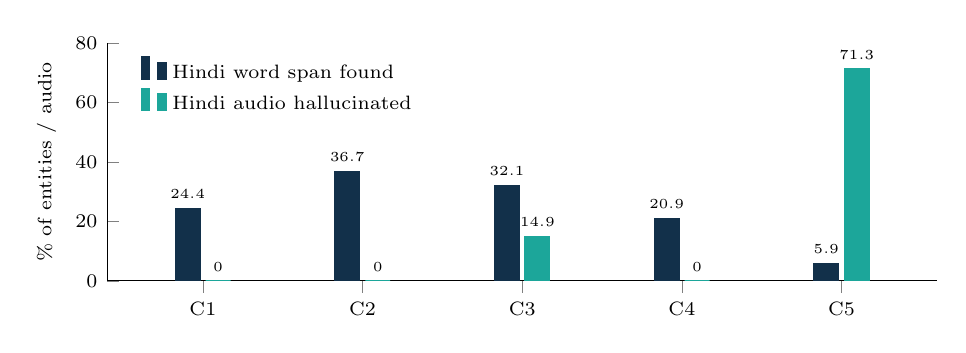
\begin{tikzpicture}
\begin{axis}[ybar,
  width=\columnwidth,
  height=4.6cm,
  bar width=9pt,
  symbolic x coords={C1,C2,C3,C4,C5},
  xtick=data,
  ymin=0,
  ymax=80,
  ylabel={\% of entities / audio},
  nodes near coords,
  nodes near coords style={font=\tiny},
  tick label style={font=\scriptsize},
  label style={font=\scriptsize},
  enlarge x limits=0.15,
  legend style={font=\scriptsize,at={(0.03,0.97)},anchor=north west,draw=none},
  legend cell align=left,
  axis x line*=bottom,
  axis y line*=left]
\addplot[fill=c12304A,draw=c12304A] coordinates {(C1,24.4) (C2,36.7) (C3,32.1) (C4,20.9) (C5,5.9)};
\addlegendentry{Hindi word span found}
\addplot[fill=c1CA69A,draw=c1CA69A] coordinates {(C1,0.0) (C2,0.0) (C3,14.9) (C4,0.0) (C5,71.3)};
\addlegendentry{Hindi audio hallucinated}
\end{axis}
\end{tikzpicture}
\caption{Per-case word-level projection rate and share of Hindi audio hallucinated by Whisper.}\label{fig:align}
\end{figure}

\subsection{ASR Quality}
Table~\ref{tab:asr} reports Whisper's failure modes. The Hindi pass hallucinated on two of the five recordings, covering 71.3\% of the audio of C5, where 27 of 31 Hindi segments are repetition loops. The English translation pass is affected more often: in four recordings, 20–49\% of English segments lie inside repetition loops, such as the question “Do you ever get diabetes at home?” repeated four times in C5.

\begin{table}[!t]
\centering\footnotesize
\caption{Whisper hallucination by recording}\label{tab:asr}
\begin{tabular}{lrrr}
\toprule
\textbf{Case} & \textbf{Hindi seg. halluc.} & \textbf{Hindi audio halluc.} & \textbf{English seg. in loops} \\
\midrule
C1 & 0/65 & 0.0\% & 40/95 (42.1\%) \\
C2 & 0/56 & 0.0\% & 28/74 (37.8\%) \\
C3 & 1/29 & 14.9\% & 0/70 (0.0\%) \\
C4 & 0/80 & 0.0\% & 14/70 (20.0\%) \\
C5 & 27/31 & 71.3\% & 42/85 (49.4\%) \\
\bottomrule
\end{tabular}
\end{table}

\subsection{Error Propagation}
Fig.~\ref{fig:err} attributes the 34 abstentions to pipeline stages. Twenty fields (58.8\%) never appear in either transcript, five (14.7\%) appear in the Hindi transcript but are lost in translation, and nine (26.5\%) reach the English transcript but are not matched by any question cue. No field was lost in answer parsing. In total, 25 of 34 misses (73.5\%) occur before any language processing, which indicates that improving ASR would raise coverage more than refining the extraction rules.

\begin{figure}[!t]
\centering
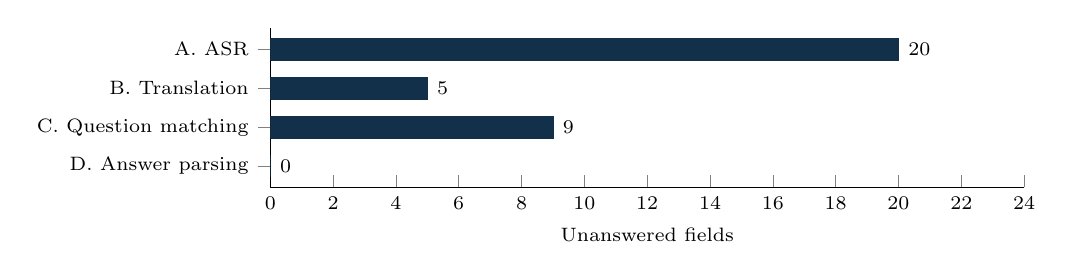
\begin{tikzpicture}
\begin{axis}[xbar,
  width=0.92\columnwidth,
  height=3.6cm,
  bar width=8pt,
  symbolic y coords={A. ASR,B. Translation,C. Question matching,D. Answer parsing},
  ytick=data,
  y dir=reverse,
  xmin=0,
  xmax=24,
  xlabel={Unanswered fields},
  nodes near coords,
  nodes near coords style={font=\scriptsize},
  tick label style={font=\scriptsize},
  label style={font=\scriptsize},
  enlarge y limits=0.18,
  axis x line*=bottom,
  axis y line*=left]
\addplot[fill=c12304A,draw=c12304A] coordinates {(20,A. ASR) (5,B. Translation) (9,C. Question matching) (0,D. Answer parsing)};
\end{axis}
\end{tikzpicture}
\caption{Pipeline stage at which each of the 34 unanswered fields was lost.}\label{fig:err}
\end{figure}

\subsection{Case Study: Family History}
In C5 the clinician asks “Did anyone get cancer at home?” and the patient replies “No. It happened in a relative.” The earlier system labelled the cancer mention inside the question PRESENT and created five duplicate family-history relations that contradicted the form's ABSENT value. The revised system labels the question mention UNKNOWN, produces one relation reconciled with the form answer, and flags the field for clinician review because the answer both denies family history and names a relative. The reference form records the same ambiguity (“No, relative reported at end”).

\section{Discussion and Limitations}
\textbf{Small, imbalanced data.} Four matched cases and two positive labels cannot support claims of generalisation or of sensitivity to symptoms. The first priority is more recordings, including patients with positive findings, and a held-out test split.

\textbf{Upstream errors dominate.} Three quarters of the misses originate in ASR or translation. A larger or Indic-specific ASR model, voice-activity detection and chunking to suppress hallucination, and a dedicated MT system instead of Whisper's translate mode are the most promising improvements.

\textbf{Rule-based NER.} Rules are transparent and every prediction is traceable, which suits a clinical review tool, but recall is limited by the lexicon. With the gold annotations now being built, fine-tuning a multilingual encoder such as MuRIL~\cite{muril} becomes feasible.

\textbf{Partial projection.} Only 28.3\% of clinical entities reach word-level alignment. A larger lexicon or neural word alignment~\cite{simalign} could raise this, and native Hindi NER would remove the dependence on translation. Finally, doctor and patient turns are inferred from question form, not from speaker diarization.

\section{Ethics and Responsible Use}
The recordings and forms contain personal health information. Processing runs entirely on the local machine, the dashboard binds only to the loopback interface, and this paper refers to cases by pseudonymous identifiers. Raw audio, transcripts and generated records must be kept out of public repositories and used only within the consent and approval obtained for the project. The system is a documentation aid, not a diagnostic device: every generated form must be reviewed by a qualified clinician, and UNKNOWN must never be read as a negative finding.

\section{Conclusion}
We built a transparent pipeline that turns Hindi and code-mixed screening consultations into evidence-linked forms and projects every extracted entity back to its Hindi source words. On the available data, the system is correct whenever it answers but answers only 39.3\% of the fields. Trivial baselines show that the reference set cannot reward careful extraction over guessing “no”, and the error-propagation analysis locates most of the remaining errors in speech recognition rather than in language processing. Better Hindi ASR, more and more varied recordings, and the completed NER gold standard are the next steps.

\begin{thebibliography}{99}
\bibitem{aci} W. Yim, Y. Fu, A. Ben Abacha, N. Snider, T. Lin, and M. Yetisgen, “ACI-BENCH: A novel ambient clinical intelligence dataset for benchmarking automatic visit note generation,” \emph{Sci. Data}, vol. 10, Art. no. 586, 2023.
\bibitem{careless} A. Koenecke, A. S. G. Choi, K. X. Mei, H. Schellmann, and M. Sloane, “Careless Whisper: Speech-to-text hallucination harms,” in \emph{Proc. ACM Conf. Fairness, Accountability, and Transparency (FAccT)}, 2024.
\bibitem{negex} W. W. Chapman, W. Bridewell, P. Hanbury, G. F. Cooper, and B. G. Buchanan, “A simple algorithm for identifying negated findings and diseases in discharge summaries,” \emph{J. Biomed. Inform.}, vol. 34, no. 5, pp. 301–310, 2001.
\bibitem{context} H. Harkema, J. N. Dowling, T. Thornblade, and W. W. Chapman, “ConText: An algorithm for determining negation, experiencer, and temporal status from clinical reports,” \emph{J. Biomed. Inform.}, vol. 42, no. 5, pp. 839–851, 2009.
\bibitem{whisper} A. Radford, J. W. Kim, T. Xu, G. Brockman, C. McLeavey, and I. Sutskever, “Robust speech recognition via large-scale weak supervision,” in \emph{Proc. 40th Int. Conf. Mach. Learn. (ICML)}, 2023, pp. 28492–28518.
\bibitem{metamap} A. R. Aronson, “Effective mapping of biomedical text to the UMLS Metathesaurus: The MetaMap program,” in \emph{Proc. AMIA Symp.}, 2001, pp. 17–21.
\bibitem{ctakes} G. K. Savova \emph{et al.}, “Mayo clinical Text Analysis and Knowledge Extraction System (cTAKES): Architecture, component evaluation and applications,” \emph{J. Am. Med. Inform. Assoc.}, vol. 17, no. 5, pp. 507–513, 2010.
\bibitem{umls} O. Bodenreider, “The Unified Medical Language System (UMLS): Integrating biomedical terminology,” \emph{Nucleic Acids Res.}, vol. 32, suppl. 1, pp. D267–D270, 2004.
\bibitem{i2b2} Ö. Uzuner, B. R. South, S. Shen, and S. L. DuVall, “2010 i2b2/VA challenge on concepts, assertions, and relations in clinical text,” \emph{J. Am. Med. Inform. Assoc.}, vol. 18, no. 5, pp. 552–556, 2011.
\bibitem{yarowsky} D. Yarowsky, G. Ngai, and R. Wicentowski, “Inducing multilingual text analysis tools via robust projection across aligned corpora,” in \emph{Proc. 1st Int. Conf. Human Lang. Technol. Res. (HLT)}, 2001.
\bibitem{mayhew} S. Mayhew, C.-T. Tsai, and D. Roth, “Cheap translation for cross-lingual named entity recognition,” in \emph{Proc. Conf. Empirical Methods Natural Lang. Process. (EMNLP)}, 2017.
\bibitem{simalign} M. Jalili Sabet, P. Dufter, F. Yvon, and H. Schütze, “SimAlign: High quality word alignments without parallel training data using static and contextualized embeddings,” in \emph{Findings Assoc. Comput. Linguistics: EMNLP}, 2020.
\bibitem{gliner} U. Zaratiana, N. Tomeh, P. Holat, and T. Charnois, “GLiNER: Generalist model for named entity recognition using bidirectional transformer,” in \emph{Proc. Conf. North Amer. Chapter Assoc. Comput. Linguistics (NAACL)}, 2024.
\bibitem{muril} S. Khanuja \emph{et al.}, “MuRIL: Multilingual representations for Indian languages,” 2021, \emph{arXiv:2103.10730}.
\bibitem{ratcliff} J. W. Ratcliff and D. E. Metzener, “Pattern matching: The gestalt approach,” \emph{Dr. Dobb’s J.}, vol. 13, no. 7, p. 46, Jul. 1988.
\bibitem{chrf} M. Popović, “chrF: Character n-gram F-score for automatic MT evaluation,” in \emph{Proc. 10th Workshop Statistical Mach. Transl. (WMT)}, 2015, pp. 392–395.
\bibitem{hripcsak} G. Hripcsak and A. S. Rothschild, “Agreement, the F-measure, and reliability in information retrieval,” \emph{J. Am. Med. Inform. Assoc.}, vol. 12, no. 3, pp. 296–298, 2005.
\bibitem{cohen} J. Cohen, “A coefficient of agreement for nominal scales,” \emph{Educ. Psychol. Meas.}, vol. 20, no. 1, pp. 37–46, 1960.
\bibitem{landis} J. R. Landis and G. G. Koch, “The measurement of observer agreement for categorical data,” \emph{Biometrics}, vol. 33, no. 1, pp. 159–174, 1977.
\end{thebibliography}

\end{document}
